\documentclass{standalone}
\usepackage{bm}
\usepackage{amsmath}
\usepackage{amssymb}
\usepackage{dutchcal}
\usepackage{tikz}
\usetikzlibrary{shapes.multipart}
\usetikzlibrary{decorations.pathmorphing}
\usetikzlibrary{decorations.markings}
\usetikzlibrary{patterns}
\usetikzlibrary{calc}
\usetikzlibrary{math}
\usetikzlibrary{fpu}
\usepackage{xcolor}
\definecolor{myGreen}{rgb}{0.2,0.72,0.2}
\definecolor{greengray}{rgb}{0.7,0.8,0.7}
\definecolor{bluegray}{rgb}{0.7,0.7,0.85}
\definecolor{redgray}{rgb}{0.85,0.7,0.7}
\definecolor{myWhite}{rgb}{0.98,0.98,0.98}
\definecolor{myGray}{rgb}{0.7,0.7,0.75}
\definecolor{myGold}{rgb}{0.8,0.64,0.24}

%%%%%%%%%%%%%%%%%%%%%CODE FROM INTERNET FOR GRID WITH COORDIATES%%%%
\makeatletter
\def\grd@save@target#1{%
  \def\grd@target{#1}}
\def\grd@save@start#1{%
  \def\grd@start{#1}}
\tikzset{
  grid with coordinates/.style={
    to path={%
      \pgfextra{%
        \edef\grd@@target{(\tikztotarget)}%
        \tikz@scan@one@point\grd@save@target\grd@@target\relax
        \edef\grd@@start{(\tikztostart)}%
        \tikz@scan@one@point\grd@save@start\grd@@start\relax
        \draw[minor help lines] (\tikztostart) grid (\tikztotarget);
        \draw[major help lines] (\tikztostart) grid (\tikztotarget);
        \grd@start
        \pgfmathsetmacro{\grd@xa}{\the\pgf@x/1cm}
        \pgfmathsetmacro{\grd@ya}{\the\pgf@y/1cm}
        \grd@target
        \pgfmathsetmacro{\grd@xb}{\the\pgf@x/1cm}
        \pgfmathsetmacro{\grd@yb}{\the\pgf@y/1cm}
        \pgfmathsetmacro{\grd@xc}{\grd@xa + \pgfkeysvalueof{/tikz/grid with coordinates/major step}}
        \pgfmathsetmacro{\grd@yc}{\grd@ya + \pgfkeysvalueof{/tikz/grid with coordinates/major step}}
        \foreach \x in {\grd@xa,\grd@xc,...,\grd@xb}
        \node[anchor=north] at (\x,\grd@ya) {\pgfmathprintnumber{\x}};
        \foreach \y in {\grd@ya,\grd@yc,...,\grd@yb}
        \node[anchor=east] at (\grd@xa,\y) {\pgfmathprintnumber{\y}};
      }
    }
  },
  minor help lines/.style={
    help lines,
    step=\pgfkeysvalueof{/tikz/grid with coordinates/minor step}
  },
  major help lines/.style={
    help lines,
    line width=\pgfkeysvalueof{/tikz/grid with coordinates/major line width},
    step=\pgfkeysvalueof{/tikz/grid with coordinates/major step}
  },
  grid with coordinates/.cd,
  minor step/.initial=.2,
  major step/.initial=1,
  major line width/.initial=2pt,
}
\newcommand{\Ds}{\displaystyle}

\begin{document}
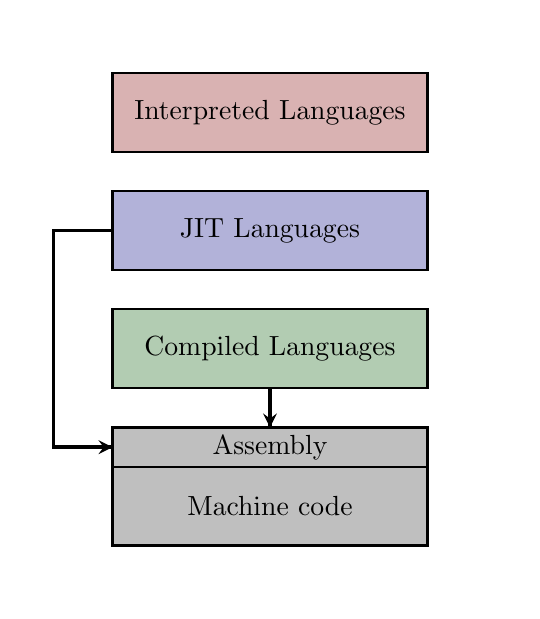
\begin{tikzpicture}
%\draw[step=.5cm] (-3,-3) to[grid with coordinates] (3,3);
\tikzmath{\s = 1.5;}

%%%%%%%%%%%%%%%%%%%%%%%%%%%%%%%%%%%%%%%%%%%%%%%%%%%%%%%%%%%%%% Setup
\coordinate (C) at (0, 0);
% just to have nice boundaries to the picture
\draw[white,fill=white] ($(-3,-4.5)$) circle (2pt);
\draw[white,fill=white] ($(+3,+2.5)$) circle (2pt);


%%%%%%%%%%%%%%%%%%%%%%%%%%%%%%%%%%%%%%%%%%%%%%%%%%%%%%%%%%%%%% Diag-1

\draw[thick, black, fill=redgray] ($(C)+(-2.0,1.0)$) rectangle ($(C)+(2.0,2.0)$);
\node[] at ($(C)+(0,1.5)$) {Interpreted Languages};

\draw[very thick, postaction={decorate, decoration={
    markings,
    mark=at position 1 with {\arrow{stealth}}}}] ($(C)+(-2.0,0.0)$) --  ($(C)+(-2.75,0.0)$) -- ($(C)+(-2.75,-2.75)$) -- ($(C)+(-2.0,-2.75)$);

\draw[thick, black, fill=bluegray] ($(C)+(-2.0,-0.5)$) rectangle ($(C)+(2.0,0.5)$);
\node[] at ($(C)+(0,0)$) {JIT Languages};

\draw[very thick, postaction={decorate, decoration={
    markings,
    mark=at position 1 with {\arrow{stealth}}}}] ($(C)+(0,-2)$) -- ($(C)+(0,-2.5)$);

\draw[thick, black, fill=greengray] ($(C)+(-2.0,-2.0)$) rectangle ($(C)+(2.0,-1)$);
\node[] at ($(C)+(0,-1.5)$) {Compiled Languages};

\draw[thick, black, fill=lightgray] ($(C)+(-2.0,-3.0)$) rectangle ($(C)+(2.0,-2.5)$);
\node[] at ($(C)+(0,-2.75)$) {Assembly};


\draw[thick, black, fill=lightgray] ($(C)+(-2.0,-4.0)$) rectangle ($(C)+(2.0,-3.0)$);
\node[] at ($(C)+(0,-3.5)$) {Machine code};






\end{tikzpicture}
\end{document}